%%%%%%%%%%%%%%%%%%%%%%%%%%%%%%%%%%%%%%%%%%%%%%%%%%%%%%%%%%%%%%%%%%%%%%%
%%%%%%%%%%%%%%%%%%%%%%%%%%%%%%%%%%%%%%%%%%%%%%%%%%%%%%%%%%%%%%%%%%%%%%%
%%%%%                                                                 %
%%%%%     04_vectorial.tex                                            %
%%%%%                                                                 %
%%%%% Author:      <author>                                           %
%%%%% Created:     <date>                                             %
%%%%% Description: <description>                                      %
%%%%%                                                                 %
%%%%%%%%%%%%%%%%%%%%%%%%%%%%%%%%%%%%%%%%%%%%%%%%%%%%%%%%%%%%%%%%%%%%%%%
%%%%%%%%%%%%%%%%%%%%%%%%%%%%%%%%%%%%%%%%%%%%%%%%%%%%%%%%%%%%%%%%%%%%%%%


\chapter{ISA Extensions}

\label{chapter:vectorial}

%The vectorial unit is supposed to increase the performance of the core when
%sub-word workloads are executed, e.g. operations on 8 or 16 bit numbers. Since
%\orion implements the 32 bit ISA of OpenRISC, it is possible to segment the data
%path, i.e. support 4x 8 bit or 2x 16 bit operations on the same data path
%without increasing the area of the data path by a significant amount.

%The OpenRISC specifications already contain a proposal for a vectorial
%extension on 64 bit \cite{OR1KSPEC}, called ORVDX64. We only have a 32 bit
%implementation and wanted to keep it that way, thus using ORVDX64 without
%modifications was not an option. Although we still used ORVDX64 as a basis for
%our own vectorial extension, adapted it to 32 bit, removed some instructions
%from it and added others.

This chapter describes the \gls{ISA} extensions that were integrated during this
thesis. Four sets of extensions were done, the first being a vectorial
extension to the \gls{ALU} which is detailed in Section~\ref{sec:vectorial}.
Section~\ref{sec:multiplier} explains the improvements to the \gls{MAC} unit of
the core. This includes adding vectorial support to the multiplier, sub-word
selection and more general multiply-accumulate instructions.
In Section~\ref{sec:misaligned_access} the misaligned memory access
implementation is explained.
Finally Section~\ref{sec:bit_count} explains the added bit counting instructions.

An overview over the encoding, mnemonics and semantic of the modified \gls{ISA}
is available in Appendix~\ref{chap:instr_encoding}.

\section{Vectorial Unit}
\label{sec:vectorial}

Our vectorial instructions extend the \gls{ALU} operations of the original
OpenRISC \gls{ISA}. In general every \gls{ALU} operation has two input operands
and one result that is stored in the general-purpose register file. There are
certain exceptions where an operation only has one input operand, e.g. for
example absolute number calculation which only needs one input operand.

\clearpage
For all instructions that take two operands, we have added six instruction
forms:

\begin{table}[H]
 \caption{Vectorial instruction forms.}
 \label{tab:vectorial_instr_forms}
 \centering\begin{tabular}{@{}lrl@{}} \toprule
  \textbf{Mnemonic} & \textbf{Width} & \textbf{Note} \\ \midrule
  lv.inst.h         & 16 bit         &  \\
  lv.inst.h.sc      & 16 bit         & scalar replication of operand B register \\
  lv.inst.h.sci     & 16 bit         & scalar replication of operand B immediate  \\
  lv.inst.b         &  8 bit         &  \\
  lv.inst.b.sc      &  8 bit         & scalar replication of operand B register \\
  lv.inst.b.sci     &  8 bit         & scalar replication of operand B immediate \\
  \bottomrule
 \end{tabular}
\end{table}

Scalar replication modifies the second operand of the instructions by
replicating the lower half word two times for the 16 bit case and the lowest
byte four times for the 8 bit case, i.e. it performs the following:
\begin{align*}
  opB[31:0] &= \{rB[15:0], rB[15:0]\} &\text{; 16 Bit case}\\
  opB[31:0] &= \{rB[7:0], rB[7:0], rB[7:0], rB[7:0]\} & \text{; 8 Bit case}\\
\end{align*}

Instead of replicating the register, the \textit{.sci} form replicates the
immediate encoded in the instruction. We have used an 8 bit wide immediate for
our vectorial instructions. For the 8 bit case the immediate is used directly,
while for the 16 bit case the immediate is sign-extended.

In the following sections an overview of the different \gls{ALU} operations is
given with details on how they were implemented.


\subsection{Addition / Subtraction / Average}

Addition and subtraction are the most basic features of an \gls{ALU} and among
the most used operations on 8 and 16 bit data types. Another common operation is
the average of two numbers, so we added support for this operation in our data
path as well. Averages were not supported in the original OpenRISC
specifications.

Figure~\ref{fig:alu_add_vec} shows the implementation of the vectorial addition,
subtraction and average. The same data path can be used for 8, 16 and 32 bit
operations. The only overhead introduced by vectorial instructions four 1-bit
wide multiplexers that are placed between the 8 bit adder slices and take care
of handling the carry bit correctly between the different slices.  On the right
hand side of this figure the additional hardware that was needed to perform
averages is shown. An average is computed by first adding the two operands and
then performing an arithmetic right shift by one bit. Note that the arithmetic
right shift performs a division by 2 towards negative infinity.

\begin{figure}[htbp]
  \centering
  \includegraphics[height=1.0\textwidth,angle=270]{./figures/alu_add_vec}
  \caption{Vectorial addition/subtraction.}
  \label{fig:alu_add_vec}
\end{figure}

% lv.add
% lv.sub
% lv.avg

\subsection{Minimum / Maximum / Absolute Value}

Calculating minimum, maximum and absolute values is important for many
applications. Using the standard OpenRISC instruction set those operations need
a lot of instructions including branches. 
Our main interest lay on vectorial instructions, but since we wanted those
instructions for the vectorial unit, we were able to also add them to the normal
integer pipeline without any additional cost, thus we introduced the following
instructions that were not part of the original OpenRISC instruction set:
\instr{l.min}, \instr{l.max} and \instr{l.abs}.

Figure~\ref{fig:max_inst} shows a comparisons of assembler instructions
necessary to perform a maximum computation. On the left an optimized maximum
computation based on the original OpenRISC specifications can be found. Note
that a compiler would usually use at least five instructions to perform the
same operation as it is not able to put the first addition into the delay slot.
On the right hand side the same functionality is shown with our new max
instruction.  When we consider many maximum calculations on sub-word integers,
the strength of having a dedicated maximum instruction gets even more pronounced
because the vectorial version can be used.

% Create an enviroment for shell commands.
\newenvironment{shellenv2}%
{%
   \begin{Sbox}\begin{minipage}{\textwidth}\begin{texttt}%
 }%
 {\end{texttt}\end{minipage}\end{Sbox}%
 \setlength{\fboxsep}{6pt}\shadowbox{\TheSbox}}%


\begin{figure}[H]
 \begin{subfigure}[b]{0.45\linewidth}
\begin{instrenv}
l.sfgts rA, rB
l.bf 0xC
l.addi rD, rA, 0
l.addi rD, rB, 0
\end{instrenv}
  \caption{Original max. computation.}
 \end{subfigure}\hfill
 \begin{subfigure}[b]{0.45\linewidth}
  \begin{instrenv}
l.max rD, rA, rB
  \end{instrenv}
  \caption{New max. instruction.}
 \end{subfigure}

 \caption{Maximum operation in assembler.}
 \label{fig:max_inst}
\end{figure}


Figure~\ref{fig:alu_minmax} shows the implementation of the min/max/abs circuit.
Since this operation was not present in the \orion core before this thesis has
started, we had to add additional hardware. Mainly what was needed was a
vectorial comparison unit (which was also needed for vectorial comparison
operations) and a multiplexer on 32 bit.

If we consider only the maximum operation, the circuit works as follows.
The two operands, \textit{op\_a} and \textit{op\_b}, are fed into a vectorial
comparison unit that is configured based on the vectorial mode (8, 16 or 32 bit)
and signed mode. The output of the vectorial comparator is then used to set the
multiplexers to the correct setting and select the bigger of the two operands.
This works almost exactly the same way for minimum, the only difference being
that the output of the vectorial comparator is inverted and thus instead of the
bigger of the two operands the smaller is chosen.

To perform an absolute value calculation, we reuse the subtraction of the
vectorial adder that was described above. In this case \textit{op\_a} is the
operand data, while \textit{op\_b} is set to 0. The adder then computes $0 -
\textit{op\_a}$ and supplies this result to \textit{res\_sub}.  The vectorial
comparator compares \textit{op\_a} and 0, and using this result we can select
either \textit{op\_a} or $-\textit{op\_a}$ with the multiplexers.

\begin{figure}[htbp]
  \centering
  \includegraphics[height=1.0\textwidth,angle=270]{./figures/alu_minmax}
  \caption{Vectorial min/max/abs.}
  \label{fig:alu_minmax}
\end{figure}




\subsection{Shifts}

Similar to other implementations \cite{PLX,MAX2} we wanted to support vectorial shift
instructions because a considerable part of today's workloads involve shift
operations on sub-word data. For those instructions shifts by immediates and
shifts by values stored in registers should be supported which is a very good
fit for our instruction format described in
Table~\ref{tab:vectorial_instr_forms}.

Vectorial shift operations with scalar replication of immediates shifts all
sub-words by the same amount to the left or right. The same is true for scalar
replication of registers. But if scalar replication is not used, it is possible
to shift each sub-word of operand A by a different amount given by the sub-words
in operand B. Allowing shifts by different amounts in a vectorial operation
makes it more general and allows the use of the vectorial unit in more cases.

If shift operations would not be supported, it would sometimes be necessary to
convert the vector data type to multiple scalar data values to perform those
operations. In many cases this would ruin the performance gains that were
achieved by using other vectorial instructions.
In the end it would be better not to use vectorial instructions at all in those
cases.

%TODO: implementation


\subsection{Logical Operations}

To support logical operations for vectorial workload nothing has to be added in
hardware, since an \instr{AND} on 8 or 16 bit is identical to an \instr{AND} on
32 bit. The only difference being that our design for vectorial instructions
allows scalar replication. Since this was already implemented for other
vectorial operations, adding scalar replication for logical operations was
entirely for free in hardware.

The following logical operations have been added without any hardware overhead
except for the necessary decoding of the new instructions:
\begin{itemize}
  \item \instr{lv.and\{,.sc,.sci\}}
  \item \instr{lv.or\{,.sc,.sci\}}
  \item \instr{lv.xor\{,.sc,.sci\}} 
\end{itemize}



\section{Multiplication}
\label{sec:multiplier}

One of the most critical operations in a typical RISC pipeline is the
multiplication, its operation is far more complex than an addition and it
thus has a much higher delay, even when considering vectorial additions.

To keep the common case fast in the core, we decided to simplify the
multiplication design and try to fit it into just one cycle. The original OR1200
core used three cycles to compute a multiplication \cite{OR1200}, while the
original \orion core used two cycles because the full 64 bit result could not be
computed in a single cycle without impacting the critical path.

For the applications we are targeting the 64 bit result of a multiplication is
of minor importance, so we decided to move to a 32 bit result in order to
simplify the hardware design. Multiplying a 32 bit number with a 32 bit number
now yields the lower 32 bit of the product  in our modified ISA instead of the
full 64 bit wide product.
While we loose precision and cannot incorporate the full 64 bit result, we gain
performance as it is simpler to calculate only a 32 bit product. The 64 bit
result of a multiplication is seldom used and it is cumbersome to obtain in
OpenRISC as it is not saved in a \gls{GPR} but in a \gls{SPR}. In order to
use the result in the original OpenRISC specifications, one would have to first
move it from the \gls{SPR} to the \gls{GPR} using two \instr{l.mfspr}
instructions. As the \gls{SPR} is part of the \gls{WB} stage of the core, the
two \instr{l.mfspr} instructions may take three cycles if the result should be
used in the next cycle, this is due to a necessary pipeline stall in this case.
So together with the two cycle execution of the multiplication we end up with a
five cycle latency to compute a 64 bit result and use it for normal operations.


\subsection{(Vectorial) MAC}
The \gls{MAC} operation that is specified in OpenRISC \cite{OR1KSPEC} uses a 64
bit wide accumulator stage. Since a \gls{MAC} operation needs three input
operands to perform the operation $d \mathrel{{+}{=}} a \cdot c$, the
accumulator is kept local in the \gls{SPR} to hold the 64 bit wide operand $d$.
To transfer data between the general-purpose and the special-purpose registers a
significant overhead is required and many cycles are lost due to this, i.e. two
cycles to initialize the \gls{SPR} and two to three cycles to get the result
back to the \gls{GPR}. This is especially bad when only one \gls{MAC} operation
on 32 bits is required, in this case it is better to just perform a
multiplication and a subsequent addition in two separate instructions instead of
using the dedicated \gls{MAC} instruction which would need a total of five
cycles.

In order to get rid of this issue, we added another \gls{MAC} instruction which
uses the general-purpose register as the source of the accumulator. This fits
very well with the 32 bit result of the multiplier, as the general-purpose
registers are only 32 bit wide.
By moving to this scheme and still perform one \gls{MAC} operation per cycle, we
needed a register file with three read ports, two for the operands A and B and
one for the accumulator. Since a third read port was already introduced for the
register-register store operations, this did not add any additional hardware
overhead.
%This led to a register file with three read ports and two write ports as an
%additional write port was added due to auto-incrementing loads and stores.
%This is of course larger than the normal register file in a \gls{RISC} processor
%that has only two read ports and one write port.

To get the full set of \gls{ALU} operations also in the vectorial case, there
needs to be support for performing 4x 8 bit and 2x 16 bit multiplications. The
output range of those multiplications is limited to 8 bit, 16 bit respectively,
but there are still applications that can benefit from such instructions.
As we have already decided to have a \gls{MAC} instruction that uses the
general-purpose register to store the accumulator, we could also do this for the
vectorial case.


Comparing the original OpenRISC specifications with our extension, we removed
multiply-accumulate on 64 bit with the accumulator in \gls{SPR} and use a
general-purpose register file based accumulator instead. We add vectorial
operations to the \gls{MAC} unit and allow 4x 8 bit and 2x 16 bit
multiplications in parallel.


\subsection{Sub-Word Selection}

To support multiple precision multiplications, e.g. 32 bit number times 32 bit
number with a 64 bit wide product, in an efficient manner, we needed some additional
instructions. Getting a 64 bit result for a 32 bit x 32 bit multiplication was
easy with the original OpenRISC specifications, but not so simple anymore when
we have limited the output range of the multiplier to the lower 32 bit.

To mitigate this issue, sub-word selection for multiplications was introduced.
With only a 32 bit multiplication result, full precision can only be achieved
when 16 bit input operands are used. To calculate a 64 bit multiplication
product, four partial products have to be computed and added in subsequent
steps. Figure~\ref{fig:mul64_instructions} shows the assembler instructions
necessary to perform the 64 bit multiplication.
Figure~\ref{fig:mul64_original} shows the case when we follow the OpenRISC
specifications which needs at least four cycles to execute, depending on
pipeline stalls of the implementation.
Figure~\ref{fig:mul64_wo_spr} shows the case when we use only a 32 bit result of
the multiplier. To compute the 64 bit product four 32 bit wide partial products
are needed. Each partial product is computed by performing one 16 bit times 16
bit multiplication. The four partial products are then shifted accordingly and
accumulated. Since the result spans two general-purpose registers, care must be
taken to handle the carry between the two 32 bit registers correctly. This
computation needs 16 instructions in total and thus 16 cycles are required.

Sub-word selection allows us to select the lower or upper 16 bits of both input
operands of the multiplier before performing the multiplication or \gls{MAC}
operation. This means we can perform for example
$$
rC[31:0] + \big(extZ\left(rA[15:0]\right) \cdot extS\left(rB[31:16]\right)\big)
$$
in one cycle.
So if we reconsider the 64 bit multiplication from above and use sub-word
selection and the general-purpose register \gls{MAC} instruction, we can go down
to 10 instructions and thus only 10 cycles to calculate a 64 bit product.

Sub-word selection is not only useful for a 32 bit times 32 bit multiplication,
but also for much wider multiplications, i.e. multiple-precision
multiplications.

%TODO: talk about multiple-precision algorithms with the new MAC

\begin{figure}[H]
 \begin{subfigure}[b]{0.30\linewidth}
   \footnotesize
   \begin{instrenv}
l.muld  rA, rB
l.mfspr rD, MACLO
l.mfspr rE, MACHI
   \end{instrenv}
  \caption{Original.}
  \label{fig:mul64_original}
 \end{subfigure}\hfill
 \begin{subfigure}[b]{0.30\linewidth}
   \footnotesize
   \begin{instrenv}
l.andi t0, rA, 0xFFFF
l.andi t1, rB, 0xFFFF
l.sra  t2, rB, 16
l.sra  t3, rB, 16
l.mul  t4, t0, t3
l.sll  t5, t4, 16
l.sra  t4, t4, 16
l.mul  t6, t0, t1
l.mul  t7, t2, r3
l.add  t5, t5, t6
l.addc t4, t4, t7
l.mul  t6, t1, t2
l.sll  t0, t6, 16
l.sra  t1, t6, 16
l.add  t4, t4, t0
l.addc t5, t5, t1
   \end{instrenv}
  \caption{w/o SPR.}
  \label{fig:mul64_wo_spr}
 \end{subfigure}\hfill
 \begin{subfigure}[b]{0.33\linewidth}
   \footnotesize
   \begin{instrenv}
l.mul.sh.zl  t0, rA, rB
l.sll        r1, t0, 16
l.srl        r2, t0, 16
l.mac.zl.zl  r1, rA, rB
l.macc.sh.sh r2, rA, rB
l.mul.sh.zl  t0, rB, rA
l.sll        t1, t0, 16
l.srl        t0, t0, 16
l.add        r1, r1, t1
l.addc       r2, r2, t0
   \end{instrenv}
  \caption{with subword selection.}
  \label{fig:mul64_subword}
 \end{subfigure}

 \caption{64 bit multiplication with different hardware support.}
 \label{fig:mul64_instructions}
\end{figure}

Sub-word selection can also be used for vectorial operations, e.g. we have input
data arranged in two 16 bits inside one 32 bit word and we would like to
calculate a 16 bit times 16 bit multiplication with a 32 bit result. Following
the OpenRISC specifications we first have to shift the inputs by 16 bit to the
right to get only the higher 16 bits or perform an AND operation to get only the
lower 16 bits respectively. With our new feature, we can omit this pre-processing
and perform the multiplication directly, thus making it more efficient.


\subsection{Implementation}

For the implementation of the vectorial multiplier several alternatives were
evaluated, namely using a vectorial booth multiplier \cite{BoothMul}, shared
segmentation \cite{SharedSeg} and a pure behavioral specification in
SystemVerilog.


\subsubsection{Vectorial Booth Multiplier}

The circuit shown in Figure~\ref{fig:vectorial_booth_mult} is able to perform
vectorial multiplication and \gls{MAC} operations, normal 32 bit multiplications
and \gls{MAC} calculations with 32 bit result. It uses four booth multipliers
with different input and output widths. The width of the first operand of each
booth multiplier is set to 8, 16, 24 and 32 bits respectively, while the
second operand is always 8 bit wide. The output of those multipliers is a
8, 16, 24 or 32 bit number in carry save number format, i.e. two 32 bit signals
are used to represent one 32 bit number. By feeding the results of the booth
multipliers into 4:2 compressors and shifting them accordingly, we can get the
normal 32 bit result. By adjusting the multiplexers in front of the booth multipliers
and the final multiplexer before the partitioned adder correctly, we can get the 4x 8
bit and 2x 16 bit results as well. The partitioned adder then finally takes care
of performing the addition of the carry save number and transforming it into a
normal integer that can be saved into the register file later on. The
partitioned adder takes care of suppressing carries between 8 bit and 16 bit
boundaries if the 4x 8 bit or 2x 16 bit vectorial modes are used.

\begin{figure}[H]
  \centering
  \includegraphics[height=1.0\textwidth,angle=270]{./figures/booth_mult}
  \caption{Vectorial booth multiplier.}
  \label{fig:vectorial_booth_mult}
\end{figure}

The booth multiplier and 4:2 compressors were implemented by using DesignWare
components available from Synopsys \cite{DW}, specifically \texttt{DW02\_multp}
for the booth multiplier and \texttt{DW02\_tree} for the compressors. We also
tried to implement the booth multiplier and 4:2 compressors directly but the
results of using DesignWare components were a few percent better in terms of
area and delay.


\subsubsection{Shared Segmentation}

Shared segmentation is another possibility to implement a fast vectorial
multiplier. It is based on the idea to generate the partial products in the
right bit positions from the start, also in the vectorial case. For the booth
multiplier mentioned above, multiplexers and shifts are needed to align the partial
products correctly. Shared segmentation takes care of those issues at the
beginning of the calculation by emitting them in the correct bit positions of
the partial product already. This allows a simplification of the reduction step,
where the 32 partial products are reduced to the final integer. The reduction
step in shared segmentation only needs Wallace tree adders with the option to
suppress carries between 8 and 16 bit boundaries for the vectorial modes.

More details about this method can be found in \cite{SharedSeg}.

% TODO: how implemented? probably too much work for too little reward...



\subsubsection{Behavioral}

Instead of writing complex multiplier implementations in SystemVerilog, we also
tried to do a very simple implementation by specifying the vectorial multiplier
in one \texttt{always\_comb} block in SystemVerilog. By packing the complete
functionality in just one block, we leave the synthesis tool the freedom to
choose the most suitable multiplier architecture. When we started with the
comparison of the different multiplier implementations, it was not yet clear
which one would be the best. We expected a purely behavioral implementation to
be worse, but instead the results were surprisingly good.



\subsubsection{Results \& Conclusion}

The different implementations were synthesized for the 28 nm FDSOI process of
STMicroeletronics that will be used for the pulp3 chip. The slow corner on $0.6$
Volts was used for the timing analysis, see Table~\ref{tab:mult_syn} for the
results.
Baseline is the implementation that was present before we started modifying the
\gls{MAC} unit, i.e. a two-cycle \gls{MAC} with 64 bit result that writes its
result into the special-purpose registers.

It can be seen that sub-word selection adds $\sim 0.06$ ns delay to the design, which
is in the order of only one gate delay. So we decided to accept this loss in
speed for having more features. Surprisingly the behavioral implementation seems
to be the fastest and when comparing the areas of the different implementations
it is also very competitive.
This is the reason why we decided to go with the behavioral implementation, as
it has a very simple SystemVerilog implementation and it is the fastest
available.

\begin{table}[H]
 \caption{Vectorial multiplier synthesis results.}
 \label{tab:mult_syn}
 \centering\begin{tabular}{@{}llrrr@{}} \toprule
  \textbf{Design}      & \textbf{Features} & \textbf{Area \orion [kGE]} & \textbf{Area Mult. [kGE]} & \textbf{Timing} \\ \midrule
  Baseline             & OR1k spec.        &             $41.1$ &              $12.2$ &       $7.57$ ns \\
  Vec. Booth Mult.     & MAC               &             $38.5$ &              $10.7$ &       $7.83$ ns \\
  Vec. Booth Mult.     & MAC, subword      &             $38.5$ &              $11.1$ &       $7.83$ ns \\
  Shared Segmentation  & MAC               &             $39.8$ &              $13.6$ &       $7.77$ ns \\
  Shared Segmentation  & MAC, subword      &             $38.5$ &              $10.5$ &       $7.84$ ns \\
  Behavioral           & MAC               &             $38.6$ &               $8.6$ &       $7.58$ ns \\
  Behavioral           & MAC, subword      &             $38.6$ &               $8.8$ &       $7.64$ ns \\
  \bottomrule
 \end{tabular}
\end{table}



\section{Misaligned Memory Access}

\label{sec:misaligned_access}

Misaligned memory access represents the case when a memory load or store
operation is performed that is not aligned on a natural word address. Since our
whole memory subsystem is word-organized, this case is difficult to handle. This
is the reason that the OpenRISC specifications do not allow non-word aligned
memory access, or misaligned accesses as we will call them from now on. But
there are certain benefits to add support for this kind of memory transaction,
especially vectorial operations can gain a lot of performance, since it is very
probable that we compute on 8 or 16 bit data that is not aligned on a word
address. Figure~\ref{fig:unaligned_mem_access_5x5} shows a use case of
misaligned memory access where we want to put a filter on a 2D image. The
unaligned word on the right hand side needs two load words, two shifts and one
OR instruction if no misaligned accesses are supported. So in the end it might
happen that more cycles are needed to prepare the data than what we can gain
with our vectorial operations, so it might be better to stick to conventional
operations.

\begin{figure}[htbp]
  \centering
  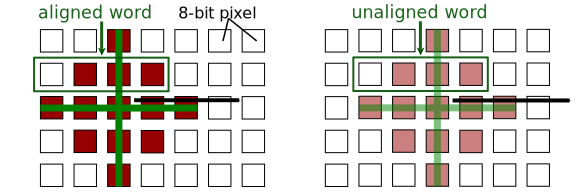
\includegraphics[width=0.7\textwidth]{./figures/unaligned_mem_access_5x5}
  \caption{2D filter with misaligned words.}
  \label{fig:unaligned_mem_access_5x5}
\end{figure}

Figure~\ref{fig:misaligned_access} shows a comparison of assembler instructions
necessary for performing a misaligned access when it is supported by the
hardware and when it is not supported. The effect on code density is immediately
visible and it is obvious that with hardware support the load can be performed
much faster.

\begin{figure}[H]
 \begin{subfigure}[b]{0.45\linewidth}
\begin{instrenv}
l.lwz  rD, 0(rA)
l.lwz  t0, 4(rA)
l.srli rD, rD, 0x1
l.slli t0, t0, 0x1
l.or   rD, rD, t0
\end{instrenv}
  \caption{w/o support.}
 \end{subfigure}\hfill
 \begin{subfigure}[b]{0.45\linewidth}
\begin{instrenv}
l.lwz rD, 1(rA)
\end{instrenv}
  \caption{with support.}
 \end{subfigure}

 \caption{Misaligned access.}
 \label{fig:misaligned_access}
\end{figure}

\gls{PULP} uses a word-aligned memory subsystem, therefor if we want to add
support for this kind of memory access, we have to do it in the core itself or
modify the memory subsystem. Preliminary trials on modifying the memory
subsystem resulted in an increase of about 10\% of our target clock period
which is not justifiable as it is only a corner case. Supporting misaligned
memory accesses in the \gls{LSU} of the core on the other hand does not impact
the timing.

Supporting misaligned memory access in the core means that two load operations
need to be performed to get the two words from the memory that contain our
misaligned word. In \orion we added support for misaligned accesses by handling
them directly in the load-and-store unit. This unit stalls the core when it
detects a misaligned load, performs the first memory access, saves the result
in a register, then performs the second load and finally assembles the complete
word from the two words. During this time the rest of the core is stalled, so
loading a misaligned word is slower than loading an aligned word, but since
everything is performed in hardware, we are only getting the delay of loading
two words and not the additional overhead of the shifts and OR operations that
are needed when there is no support in hardware. This means that in the best
case a misaligned access can be performed in just two cycles, compared to the
five cycles that were needed previously.
Of course the implementation for storing a misaligned word in memory is very
similar and also only takes two cycles in the best case.

There are not so many use cases for misaligned memory accesses in conventional
code, since the compiler always tries to align the data to natural word
boundaries. But in the case of vectorial operations, the compiler gets much more
freedom. So this is why a performance improvement can be seen by having support
for misaligned accesses when using vectorial operations.

%TODO: say that this is very important


\section{Bit Counting Instructions}

\label{sec:bit_count}

Bit counting instructions are instructions that work on the bit level of a
single word, e.g. counting the number of bits set to $1$ or $0$ in a word,
finding the first bit set to $1$ starting from the \gls{LSB} and so on.
OpenRISC \cite{OR1KSPEC} already specifies the instructions \instr{l.ff1} and
\instr{l.fl1}, but those instructions were not yet implemented in \orion.

During this thesis we added support for a couple of those kind of instructions.
Specifically we added the following instructions:

\begin{itemize}
  \item \instr{l.ff1}: Find first bit set to $1$ in a word starting from
    \gls{LSB}.
  \item \instr{l.fl1}: Find first bit set to $1$ in a word starting from
    \gls{MSB}.
  \item \instr{l.cnt}: Count the number of bits set to $1$ in a word.
  \item \instr{l.clb}: Count leading bits, the number of bits set to the same
    value as the sign bit.
\end{itemize}

It is obvious that those instructions are far more efficient than performing
those operations in the normal way using loops and branches. For example the
\instr{l.cnt} instruction would need more than 100 cycles to execute without
hardware support.

Table~\ref{tab:bit_count_syn} shows the area cost of the different
implementations compared to the baseline which does not include any of those
instructions. For this comparison the 28nm FDSOI technology from
STMicroeletronics was used. The baseline already includes the vectorial
instructions that were introduced above.
In total less than $15\%$ of the area of the \gls{ALU} is needed for all bit
counting instructions while the \gls{ALU} only occupies about $15\%$ of the area
of the core, so the area impact on the core is only about $2\%$ for all bit
counting instructions together. Similarly the bit counting instructions have no
impact on the timing properties of the core.


\begin{table}[H]
 \caption{Bit counting implementation}
 \label{tab:bit_count_syn}
 \centering\begin{tabular}{@{}lcc@{}} \toprule
   \textbf{Design}      & \textbf{Area ALU [GE]} & \textbf{ALU Percentage of Core Area} \\ \midrule
  Baseline             &           $6530$        & 13.3\% \\
  FF1, FL1             &           $6870$        & 14.0\%\\
  FF1, FL1, CLB        &           $6920$        & 14.1\%\\
  FF1, FL1, CLB, CNT   &           $7480$        & 15.3\%\\
  \bottomrule
 \end{tabular}
\end{table}

Considering a \gls{PULP} cluster with four cores, the area impact of bit counting
instructions becomes completely negligible. Such a cluster needs an area of
around $1500$ kGE, while all bit counting instructions together require only $1$
kGE, meaning that they have an impact of less than $0.07\%$ on the cluster area.
